%%%%%%%%%%%%%%%%%%%%%%%%%%%%%%%%%%%%%%%%%
% Szablon pracy dyplomowej
% Wydział Informatyki 
% Zachodniopomorski Uniwersytet Technologiczny w Szczecinie
% autor Joanna Kołodziejczyk (jkolodziejczyk@zut.edu.pl)
% Bardzo wczesnym pierwowzorem szablonu był
% The Legrand Orange Book
% Version 2.1 (26/09/2018)
%
% Modifications to LOB assigned by %JK
%%%%%%%%%%%%%%%%%%%%%%%%%%%%%%%%%%%%%%%%%

%----------------------------------------------------------------------------------------
%	CHAPTER 1
% 	author: Joanna Kolodziejczyk (jkolodziejczyk@zut.edu.pl)
%----------------------------------------------------------------------------------------

\chapter{Wprowadzenie teoretyczne}
\chaptermark{Wprowadzenie teoretyczne}

Na przestrzeni ostatnich lat zastosowanie Systemów Automatycznego Rozpoznawania Tablic Rejestracyjnych (ARTR)(ang. \textit{Automatic Licence Plate Recognition} - ALPR) stało się znacznie bardziej powszechne.
W większości dużych miast istnieją parkingi, gdzie po umieszczeniu opłaty za postój, przy zbliżeniu się do wyjazdu, szlaban otwiera się automatycznie po rozpoznaniu numeru rejestracyjnego pojazdu, którym się poruszamy.
W obecnych czasach wszystkie nowoczesne systemy do zarządzania i sterowania ruchem drogowym oparte są o technologie ARTR.
Instytucje takie jak służby drogowe, dzięki rejestrowanym i przetwarzanym w czasie rzeczywistym ogromnym ilościom danych, są w stanie odpowiednio szybko reagować na wydarzenia na drogach takie jak kolizje, korki lub innego rodzaju utrudnienia.
Innym z możliwych przykładów zastosowania wspomnianych systemów są odcinkowe pomiary prędkości, opłaty za przejazd płatnymi drogami lub wykrywanie kierowców łamiących przepisy.
Dzięki nieustannemu rozwojowi technologii i co raz wydajniejszym komputerom, systemy stają się tańszą i łatwiej dostępną alternatywą dla systemów opartych na RFID (ang. \textit{Radio-frequency identification}), które to wymagają specjalnej etykiety do prawidłowego działania.

Rozpoznawanie tablic rejestracyjnych jest techniką polegająca na wykryciu i odczytaniu znaków z tablicy rejestracyjnych na podstawie zarejestrowanego obrazu.
Do tego celu wykorzystywany jest aparat o wysokiej rozdzielczości oraz odpowiedni program komputerowy.
Oprogramowanie otrzymuje na wejściu cyfrową reprezentację obrazu.
Dla zdjęć kolorowych każdy piksel opisany jest wartościami z palety barw RGB reprezentującymi jego barwę oraz współrzędnymi umiejscowienia w obrazie.
Dla zdjęć monochromatycznych barwy opisywane są najczęściej za pomocą wartości luminacji obrazu.

W procesie automatycznego rozpoznawania tablic rejestracyjnych pozyskany obraz jest odpowiednio przetwarzany.
W procesie tym można wyróżnić trzy etapy \cite{1688109}:
\begin{itemize}
    \item \textbf{detekcję} - określenie położenia tablicy rejestracyjnej w analizowanym obrazie
    \item \textbf{segmentację} - wyodrębnienie pojedynczych znaków na fragmencie obrazu ze zlokalizowaną tablicą
    \item \textbf{identyfikację} - rozpoznanie każdego ze znaków i przedstawienie ich w formie tekstowej, którą można później wykorzystać do dalszych działań w zależności od przeznaczenia systemu
\end{itemize}

Na rysunku \ref{fig:schemat_lpr} przedstawiono graficzną reprezentację powyższego procesu.

\begin{figure}[!ht]
    \centering
    %\vspace{2mm}
    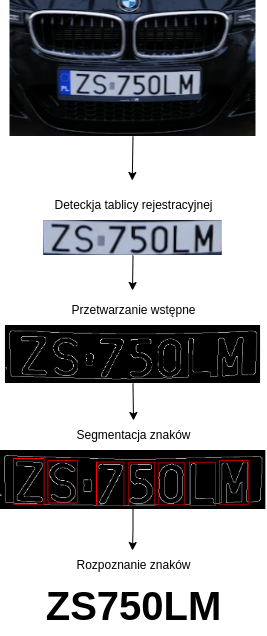
\includegraphics[scale=0.6]{Pictures/schemat_lpr.png}
    \caption{Etapy procesu automatycznego rozpoznawania tablic rejestracyjncyh (źródło:)}
    \label{fig:schemat_lpr}
\end{figure}

Kolejne etapy korzystają z wyników uzyskanych w poprzednich krokach, co oznacza, że błąd powstały we wcześniejszej fazie, będzie rzutował na jakość działania całego systemu.
W wielu systemach zanim dojdzie do rozpoznawania tablicy rejestracyjnej, obraz jest wpierw odpowiednio przetwarzany.
Jednymi z najpowszechniej stosowanych czynności są skalowanie obrazu, modyfikacje jasności oraz redukcja zakłóceń.
W zależności od wymagań stawianych przed danym mechanizmem i środowiskiem jego działania, czynności te mogą znacznie się od siebie różnić.
Najbardziej podstawowe systemy wymagają, aby pojazd znajdował się nieruchomo w określonym miejscu.
Tego typu rozwiązania najczęściej stosowane są na parkingach, gdzie szlaban otwiera się po odczycie numerów rejestracyjnych pojazdu i potwierdzeniu opłaty za postój w zewnętrznej bazie danych.
Tego rodzaju systemy pracują z reguły w środowisku o niskim poziomie zakłóceń wynikających z warunków atmosferycznych i oświetlenia.
Dzisiaj na rynku znajduje się wiele komercyjnych rozwiązań, które oferują wysoką dokładność (powyżej 95\%).
Ten rodzaj systemów ARTR nazywany systemami statycznymi.
Dużo większą złożonością charakteryzują się systemy dynamiczne, w których znacznie większą rolę odgrywają zakłócenia wynikające ze zmiennych warunków oświetlenia.
Nie bez znaczenia zostają analizowane pojazdy poruszające się z wysokimi prędkościami, których tablice rejestracyjne mogą znajdować się w różnych sektorach obrazu.
Celem niniejszej pracy jest analizowanie obrazów pochodzących z kamery samochodowej, co zdecydowanie sprawia, że jest to system dynamiczny.
Poniżej przedstawiono najczęściej stosowane metody widzenia komputerowego w systemach ARTR.


\section{Przegląd istniejących metod detekcji tablic rejestracyjnych}
\index{Przegląd istniejących metod detekcji tablic rejestracyjnych}

Detekcja numerów rejestracyjnych jest wyzywającym zadaniem ze względu na poniższe czynniki:
\begin{itemize}
    \item tablica rejestracyjna zajmuje niewielki obszar na zdjęciu
    \item istnienie ogromnej ilości formatów tablic rejestracyjnych (w zależności od kraju rejestracji lub rodzaju pojazdu)
    \item słabe oświetlenie, rozmazany obraz
    \item ruch pojazdu, zabrudzone tablice
\end{itemize}
W związku z tym, trudno jednoznacznie stwierdzić, która z metod jest najbardziej efektywna.
Tradycyjne metody widzenia komputerowego oparte są na cechach takich jak kształt, kolor, symetria, tekstury itp.\cite{9310202}
Poniżej wyróżniono najczęściej stosowane metody w detekcji tablic rejestracyjnych.

\subsection{Metody oparte na teksturach (ang. \textit{Texture based)}}
test

\subsection{Metody oparte na krawędziach (ang. \textit{Edge based)}}
tst

\subsection{Metody oparte na kolorach (ang. \textit{Color based)}}
sas

\subsection{Metody oparte na znakach (ang. \textit{Character based)}}
asd
Niniejszy szablon powstał na bazie szablonu\footnote{\url{http://www.LaTeXTemplates.com}} o nazwie ,,The Legrand Orange Book''.
Autorzy pierwotnego stylu to:
\begin{itemize}
    \item Mathias Legrand (legrand.mathias@gmail.com)
    \item Vel (vel@latextemplates.com).
\end{itemize}

Późniejsze zmiany na potrzeby stylu Wydziału Informatyki zostały wprowadzone przez Joannę Kołodziejczyk (jkolodziejczyk@zut.edu.pl). Wizualna strona stylu jest konsensusem uzyskanym w wyniku prac zespołu:
\begin{itemize}
    \item Anna Barcz
    \item Marcin Korzeń
    \item Mirosław Łazoryszczak
    \item Piotr Piela
\end{itemize}

Niniejszy styl jest udostępniony na zasadach licencji CC BY-NC-SA 3.0 ({\url{http://creativecommons.org/licenses/by-nc-sa/3.0/}}).


\section{Kompilowanie dokumentu}
\index{Kompilacja}

Do kompilacji wykorzystać należy procesor {\em pdflatex}.

%Ten szablon wykorzystuje pakiet - menedżer spisu literatury o nazwie {\em biber}\footnote{ \url{http://biblatex-biber.sourceforge.net}}, który jest dostępny w wielu popularnych środowiskach programistycznych dla \LaTeX.

Najpewniejszym sposobem na poprawną kompilację jest wykonanie jej z wiersza poleceń następującą sekwencją rozkazów:

\begin{lstlisting}[language=bash, caption=Skrypt kompilujący, label=alg:1]
pdflatex main
biber main
pdflatex main
pdflatex main

\end{lstlisting}

Szablon wykorzystuje również rozliczne pakiety, które mogą wymagać
zaktualizowane do najnowszych wersji. Rekomendowane jest więc, by utrzymywać swoją wersję dystrybucji \LaTeX w najnowszej wersji.


\section{Zawartość pakietu}\index{Zawartość pakietu}

Pakiet ze stylem zawiera pliki tekstowe z zawartością przykładowej pracy , czyli w tym wypadku niniejszego przewodnika oraz pliki konfiguracyjne. W tabeli \ref{tab:1} znajduje się lista plików wraz z ich krótkim opisem.

\begin{table}[h]
    \centering
    \caption{Pliki w pakiecie szablonu}
    \begin{tabular}{p{.2\textwidth}|p{.1\textwidth} | p{.60\textwidth}}
        \toprule
        \textbf{Nazwa pliku} & \textbf{Edycja} & \textbf{Opis}                                                                                                                                                               \\
        \midrule
        main.tex             & TAK             & Główny plik pracy. Zawiera otwarcie dokumentu, dołącza pliki konfiguracyjne, spis treści, dołącza wszystkie rozdziały, literaturę oraz zamyka dokument.                     \\
        definitions.tex      & TAK             & Zawiera elementy strony tytułowej: autora, tytuł, niezbędne informacje ze strony tytułowej.                                                                                 \\
        abstract.tex         & TAK             & Zawartość streszczenia pracy w j. polskim i j. angielskim. Zaleca się, by nie przekroczyć tekstem 1 strony.                                                                 \\
        introduction.tex     & TAK             & Wstęp pracy dyplomowej                                                                                                                                                      \\
        chapter1.tex         & TAK             & Zawartość rozdziału pierwszego.                                                                                                                                             \\
        chapter2.tex         & TAK             & Zawartość rozdziału drugiego.                                                                                                                                               \\
        conclusions.tex      & TAK             & Zakończenie/podsumowanie pracy dyplomowej.                                                                                                                                  \\
        bibliography.bib     & TAK             & Plik z literaturą w formacie bib.                                                                                                                                           \\
        Pictures             & TAK             & Katalog zawierający ilustracje i grafiki z pracy. Nazwa katalogu jest wykorzystana w pliku konfiguracyjnym jako katalog domyślny do każdego osadzonego obiektu graficznego. \\
        title\_page.tex      & NIE             & Struktura strony tytułowej.                                                                                                                                                 \\
        structure.tex        & NIE             & Plik konfiguracyjny (preambuła). Podłącza i konfiguruje wszystkie niezbędne pakiety oraz definiuje otoczenia wykorzystywane w szablonie.                                    \\
        \bottomrule
    \end{tabular}
    \label{tab:1}
\end{table}
%------------------------------------------------

\subsection{Podstawowe wymagania dotyczące szablonu}

Praca ma ustawiony format wielkości strony A4, w pliku {\em structure.tex} w konfiguracji pakietu {\bf geometry}. Przygotowana jest do druku dwustronnego. Ustawiony jest 1cm margines na oprawę.

\noindent{\bf UWAGA!} Każdy rozdział zaczyna się na stronie nieparzystej

\subsection{Bibliografia}

Po zaktualizowaniu pliku z literaturą należy dokonać kompilacji z użyciem procesora {\em biber} a nie standardowego  {\em Bibtex}. Następnie dwukrotnie skompilować z użyciem {\em pdflatex}, aby zmiany były widoczne. Pakiet do zarządzania bibliografią to {\em biblatex}. Jego konfiguracja jest dostępna w pliku {\em structure.tex}

Bibliografia w pracach dyplomowych ma format numeryczny, sortowanie alfabetyczne i jest podzielona na części: książki, artykuły i źródła internetowe i inne. Konfiguracja jest zapisana w niniejszym szablonie.

%Tylko zacytowane prace znajdą się w spisie literatury. Nie należy tego zmieniać. Cytowanie odbywa się przez użycie polecenia $\backslash cite\{\}$ a efekt jest następujący: \cite{book_key}, \cite{article_key}, \cite{lam1994}, \cite{knuthwebsite}.





